\documentclass[conference]{IEEEtran}
\IEEEoverridecommandlockouts
% The preceding line is only needed to identify funding in the first footnote. If that is unneeded, please comment it out.
\usepackage{cite}
\usepackage{amsmath,amssymb,amsfonts}
\usepackage{algorithmic}
\usepackage{graphicx}
\usepackage{textcomp}
\usepackage[table]{xcolor}
\usepackage{url}
\usepackage{multirow}
\def\BibTeX{{\rm B\kern-.05em{\sc i\kern-.025em b}\kern-.08em
    T\kern-.1667em\lower.7ex\hbox{E}\kern-.125emX}}
\begin{document}

\title{Route Subnetwork Generation using OpenStreetMap Data for Emergency Response Problem Modelling in Indonesia
%\thanks{Identify applicable funding agency here. If none, delete this.}
}

\author{\IEEEauthorblockN{Yohanes Gultom}
\IEEEauthorblockA{\textit{Faculty of Computer Science} \\
\textit{Universitas Indonesia}\\
Depok, Indonesia \\
yohanes.gultom@ui.ac.id}
\and
\IEEEauthorblockN{Heru Suhartanto}
\IEEEauthorblockA{\textit{Faculty of Computer Science} \\
\textit{Universitas Indonesia}\\
Depok, Indonesia \\
heru@cs.ui.ac.id}
%\and
%\IEEEauthorblockN{3\textsuperscript{rd} Given Name Surname}
%\IEEEauthorblockA{\textit{dept. name of organization (of Aff.)} \\
%\textit{name of organization (of Aff.)}\\
%City, Country \\
%email address or ORCID}
%\and
%\IEEEauthorblockN{4\textsuperscript{th} Given Name Surname}
%\IEEEauthorblockA{\textit{dept. name of organization (of Aff.)} \\
%\textit{name of organization (of Aff.)}\\
%City, Country \\
%email address or ORCID}
%\and
%\IEEEauthorblockN{5\textsuperscript{th} Given Name Surname}
%\IEEEauthorblockA{\textit{dept. name of organization (of Aff.)} \\
%\textit{name of organization (of Aff.)}\\
%City, Country \\
%email address or ORCID}
%\and
%\IEEEauthorblockN{6\textsuperscript{th} Given Name Surname}
%\IEEEauthorblockA{\textit{dept. name of organization (of Aff.)} \\
%\textit{name of organization (of Aff.)}\\
%City, Country \\
%email address or ORCID}
}

\maketitle

\begin{abstract}
Route subnetwork generation is useful in modelling disaster emergency response operation problems such as evacuation, aid distribution, and personnel scheduling. Through this paper, we propose an end-to-end approach of generating subnetwork based on list of point of interests (villages, shelters, depots, etc) and publicly available data using combination of opensources tools. The end result is an opensource software available in public code repository. We also present some experiment results for three areas in Indonesia: Jakarta, Lombok, and Yogyakarta.
\end{abstract}

\begin{IEEEkeywords}
subnetwork, openstreetmap, emergency response
\end{IEEEkeywords}

\section{Introduction}

Route subnetwork generation is a process of extracting some portion of map data (eg. OpenStreetMap data) to build a network/graph where point of interest (POI) nodes are connected by minimum required routes as edges. This subnetwork is useful in efficiently modelling emergency response problems such as evacuation, aid distribution, and personnel scheduling.

The goal of the subnetwork generation is to process list of POI (POI ID, POI category, latitude, and longitude) to generate a subnetwork network/graph where:

\begin{enumerate}
\item Each nodes represents POI or route intersection
\item Each edges represents route between node
\item Only routes that are required to connect POI included
\item Each nodes has risk index (greater value means greater risk)
\item Each routes has risk index derived from its nodes' risk
\end{enumerate} 

\section{Related Works}

OpenStreetMap.org (OSM) \cite{haklay2008openstreetmap} is an open community-driven map data provider that provides standard and data needed to build a subnetwork for emergency response problem modellling. The problem is that it contains too much data so filtering and extraction are needed. 

OpenStreetMap.id is a website that provides extracted OSM data for most provinces in Indonesia in Protocolbuffer Binary Format (PBF). This website solved the issue regarding regional data extraction. 

InaRISK\cite{Bnpb2016Inarisk} is a public Geographic Information System provided by The National Agency for Disaster Countermeasure (BNPB) of Indonesia which was launched in 2016. This system provides information about the disaster risk index of all regions in Indonesia in a form of colored map layer as shown in Figure \ref{fig_jakarta_flood_risk_layer_inarisk}.

\begin{figure}
\centerline{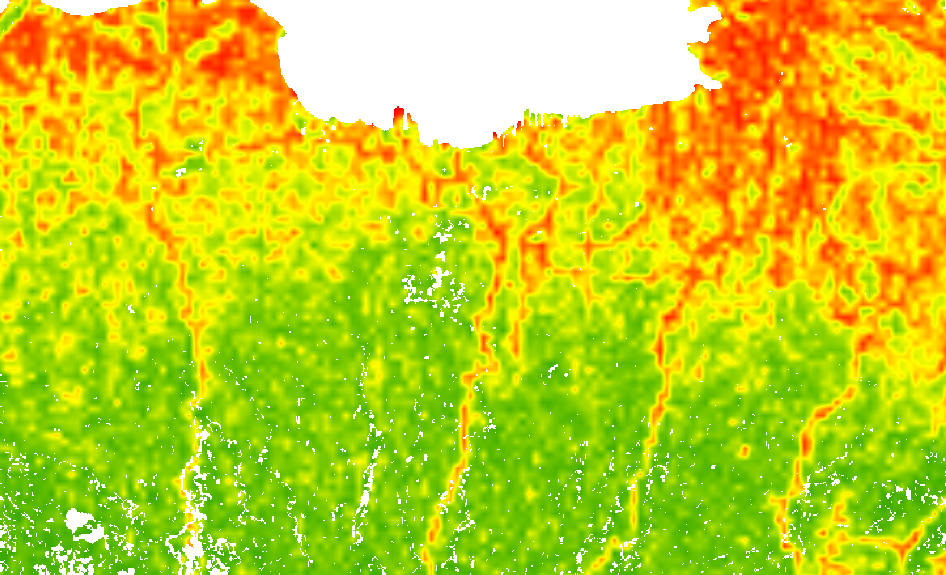
\includegraphics[scale=0.3]{jakarta_flood_risk_layer_inarisk.png}}
\caption{Jakarta flood disaster risk index from INARISK}
\label{fig_jakarta_flood_risk_layer_inarisk}
\end{figure}

OsmToRoadGraph\cite{Gemsa2017OsmToRoadGraph} is an opensource tool to generate graph/network from raw OSM data. Since the OpenStreetMap.id only provides PBF file, we will need additional tool called Osmconvert\cite{OpenStreetMap2019OsmConvert} to convert PBF to OSM before using OsmToRoadGraph to generate graph/network data in PYCGR/PYCGRC and JSON format.

PostGIS\cite{postgis2019postgis} is an spatial data extension of one of the most popular opensource database, PostgreSQL\cite{postgresql1996postgresql}. PostGIS allows us to map each POI provided by user to their nearest node in PYCGR file. The only thing left to solve is to remove unecessary nodes and routes from the graph to reduce the size of final input data for the model.

NetworkX\cite{SciPyProceedings_11} is an opensource Python package that provides data structure and APIs for complex graph search and manipulations. This package provides a way to remove unecessary nodes and routes in order to generate minimized subnetwork/subgraph suitable for modelling.


\section{Methodology}

\begin{figure*}
\centerline{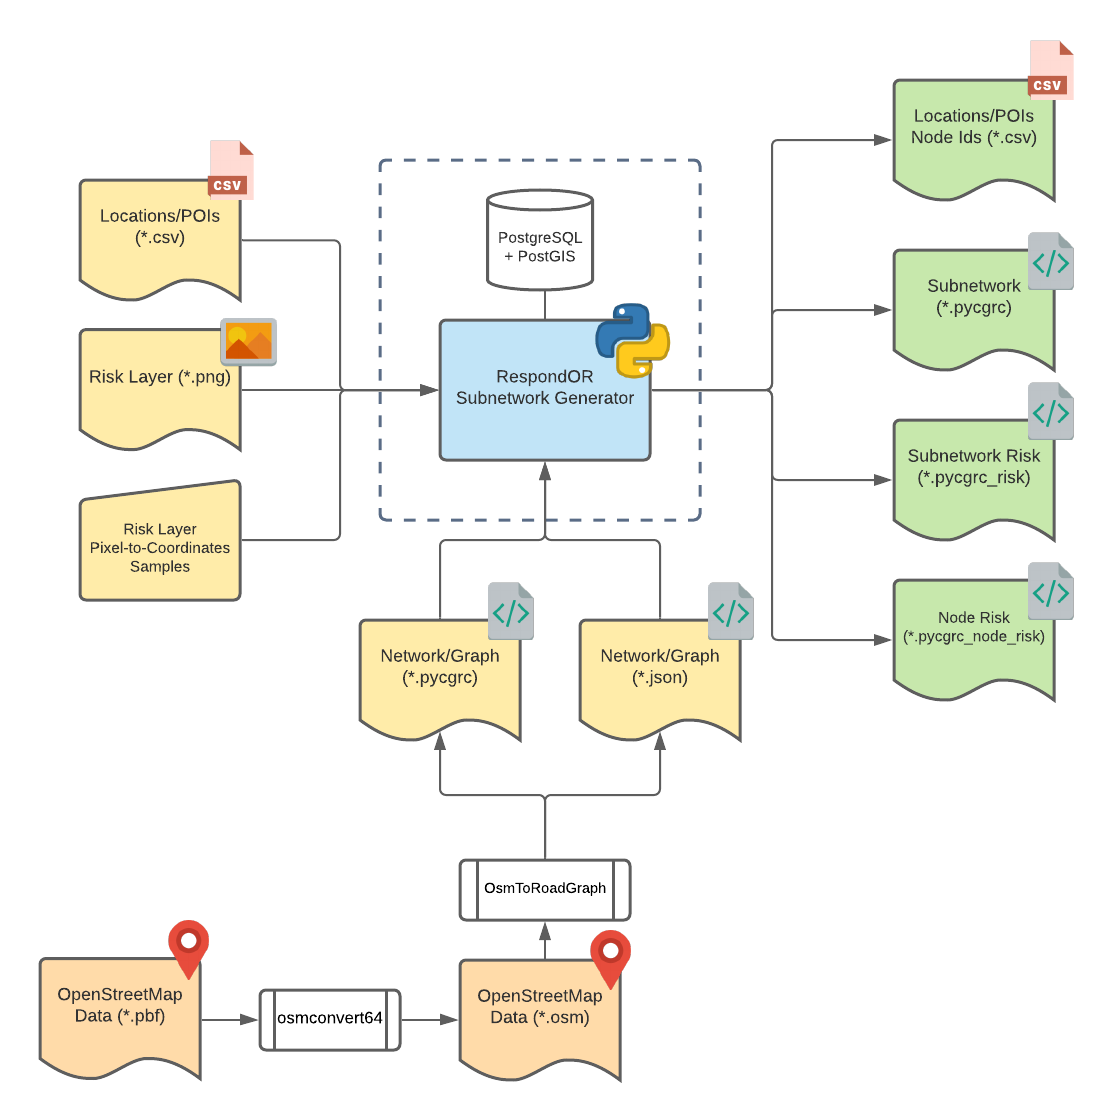
\includegraphics[scale=0.6]{system-flowchart.png}}
\caption{End-to-end network generation system flowchart}
\label{fig_system_flowchart}
\end{figure*}

In a nutshell, the methodology that we propose is combining related tools into a new system to generate route subnetwork from POI of emergency response operation. The flowchart of the system is shown in Figure \ref{fig_system_flowchart}.

Our proposed Subnetwork Generator requires five inputs (shown as yellow documents and manual input in flowchart):

\begin{enumerate}

\item \textbf{Locations/POI file (*.csv)}. This is a list of locations or point of interests in an emergency operation in Comma Separated Value (CSV) format. Each row consists of 4 columns: location name, location category (village/shelter/depot/other), latitude, longitude. For example: \texttt{ANCOL, village, -6.125215, 106.8362474}.

\item \textbf{Risk Layer (*.png)}. This is an image representing disaster risk layer downloaded from InaRISK\cite{Bnpb2016Inarisk} ArcGIS web service. The web service contains risk layers for many types of disasters (flood, earthquake, volcano eruption .etc) and for all populated areas in Indonesia. But we only need to extract only minimal area that covers the whole POI. For example we can extract flood risk layer for Jakarta as shown in Figure \ref{fig_jakarta_flood_risk_layer_inarisk} from \url{https://service1.inarisk.bnpb.go.id:6443/arcgis/rest/services/inaRISK/layer_bahaya_banjir/ImageServer}.

\item \textbf{Risk Layer Pixel-to-Coordinates Samples}. This is a list of map of pixel and coordinates pairs that will be used to estimate risk index (based on color) of coordinates (latitude, longitude) within the network (locations and routes). These samples must be obtained manually by comparing the Risk Layer and the map beneath it using InaRISK ArcGIS web service. Our generator will need at least three samples to work. The format of each sample is \texttt{[[x,y],[latitude,longitude]]}. For example: \texttt{[[199, 151], [-6.124142, 106.656685]]}.

\item \textbf{Network/Graph file (*.pycgrc)}. This is a graph representation of OpenStreetMap data generated by OsmToRoadGraph\cite{Gemsa2017OsmToRoadGraph}. It is a text file with specific format where line 1-7 contains comments, line 8 contains number of nodes, line 9 contains number of edges/routes, and the rest of the lines are respectively the nodes (ID, latitude, longitude) and the routes (source node ID, target node ID, length, street type, maximum speed, bidirectionality). The nodes included in this network/graph file don't only represent locations but also road junctions/intersections. Further details can be found in OsmToRoadGraph Github repository \url{https://github.com/AndGem/OsmToRoadGraph}.

\item \textbf{Network/Graph file (*.json)}. This is also a graph representation of OpenStreetMap data generated by OsmToRoadGraph\cite{Gemsa2017OsmToRoadGraph} but in NetworkX\cite{SciPyProceedings_11} JSON format. This input file will be used to find minimal edges/routes efficiently using NetworkX library.

\end{enumerate}

As indicated in the flowchart, the last two of the input files are the result of preprocessing the raw input, OpenStreetMap Protocolbuffer Binary Format (PBF) file, using existing tools: osmconvert\cite{OpenStreetMap2019OsmConvert} and OsmToRoadGraph\cite{Gemsa2017OsmToRoadGraph}. In the case where we can obtain the uncompressed OpenStreetMap data (*.osm) we can directly use OsmToRoadGraph to produce necessary input files.

Our proposed subnetwork generator (the only blue process in the flowchart) does the following steps to generate the route subnetwork:

\begin{itemize}


\item Loads OSM nodes name and coordinates (latitude \& longitude) from network/graph file (*.pycgrc) to PostGIS-extended PostgreSQL database

\item Loads POI list and find nearest OSM nodes using PostGIS distance operator \url{https://postgis.net/docs/geometry_distance_knn.html} 

\item Loads JSON graph and finds minimal nodes/edges required by combining shortest paths of POI permutation pairs. Since the existing shortest-path algorithm takes time to run, the processes are run in parallel utilizing multicores CPU

\item Finds risk index of each nodes by converting pixel colors in InaRISK Risk Layer image (*.png). Manually input pixel-to-coordinates samples are used to estimate the corresponding pixel for each node's coordinates (latitude/longitude)

\item Writes output files that represent the route subnetwork, risk index, and mapping to input POI

\end{itemize}

At the end of the process, our generator produces four outputs:

\begin{enumerate}

\item \textbf{Locations/POI Node Ids (*.csv)}. The nearest OpenStreetMap node IDs are mapped to each locations/POI and appended to the original CSV input file. By having these node IDs, we can link each locations/POI to subnetwork (*.pycgrc) and risk files (*.pycgrc\textunderscore node\textunderscore risk and *.pycgrc\textunderscore risk).

\item \textbf{Subnetwork (*.pycgrc)}. This is an extracted version of the original network/graph file (*.pycgrc). Our generator will create new file with the similar name but with prefix. For example if the input name is jakarta.pycgrc then the subnetwork output file wil be jakarta\textunderscore subnetwork.pycgrc.

\item \textbf{Node Risk (*.pycgrc\textunderscore risk)}. This file contains a copy of subnetwork nodes but appended with the risk index of the node (0.0-1.0) . The bigger the value is the more dangerous the route is.

\item \textbf{Subnetwork Risk (*.pycgrc\textunderscore risk)}. This file contains a copy of subnetwork edges/routes appended with additional value which is the risk index (0.0-1.0). This edge/route risk value is the mean of the source and target nodes' risk indexes.

\end{enumerate}

Additionally we also provide a simple webserver that render the subnetwork on top of interactive map (provided by https://mapbox.com) as shown in Figure \ref{fig_jakarta_subnetwork_visualized}.The networks or roads are represented by the blue line. While the villages, shelters, depots are respectively represented by yellow, green, and light blue icons. Some additional icons are also available to represent additional nodes such as damaged infrastructures, warehouses, airports .etc.

The source code of our proposed system along with its usage guide are currently published in a publicly accessible code repository https://github.com/yohanesgultom/respondor.

\section{Experiments}

\bgroup
\def\arraystretch{1.5}
\begin{table*}[htbp]
\caption{Experiment Results}
\begin{center}
\begin{tabular}{|c|l|c|c|c|c|c|}
\hline
\multicolumn{1}{|c|}{\multirow{2}{*}{\textbf{No}}} & 
\multicolumn{1}{c|}{\multirow{2}{*}{\textbf{Operation}}} & 
\multicolumn{1}{c|}{\multirow{2}{*}{\textbf{Area ($km^2$)}}} & 
\multicolumn{1}{c|}{\multirow{2}{*}{\textbf{\# POI}}} & 
\multicolumn{2}{c|}{\textbf{\% Reduction}} & 
\multirow{2}{*}{\vtop{\hbox{\strut \textbf{Avg Processing}}\hbox{\strut \textbf{Time (min)}}}} \\ 
\cline{5-6}
\multicolumn{1}{|c|}{} & 
\multicolumn{1}{c|}{} & 
\multicolumn{1}{c|}{} & 
\multicolumn{1}{c|}{} & 
\multicolumn{1}{c|}{\textbf{Nodes}} & 
\multicolumn{1}{c|}{\textbf{Routes/Edges}} & 
\multicolumn{1}{c|}{} \\ 
\hline
1 & Yogyakarta earthquake (2020)	& 32.5		& 182 & 	97.4\% & 97.5\% 	& 23.24 \\ \hline
2 & Jakarta flood (2013) 			& 661.5		& 346 & 	82.0\%	& 84.2\% 	& 26.01 \\ \hline
3 & Lombok earthquake (2018) 		& 4,725.0	& 480 & 	77.0\%	& 78.1\% 	& 166.70 \\ \hline
\end{tabular}
\label{table_experiment_results}
\end{center}
\end{table*}
\egroup

%\bgroup
%\def\arraystretch{1.5}
%\begin{table*}[htbp]
%\caption{Experiment Results}
%\begin{center}
%\begin{tabular}{|c|l|c|c|c|c|c|c|c|c|}
%\hline
%\multicolumn{1}{|c|}{\multirow{2}{*}{\textbf{No}}} & \multicolumn{1}{c|}{\multirow{2}{*}{\textbf{Operation}}} & \multicolumn{1}{c|}{\multirow{2}{*}{\textbf{\# POI}}} & \multicolumn{2}{c|}{\textbf{Full Network (input)}} & \multicolumn{2}{c|}{\textbf{Subnetwork (output)}}  & \multicolumn{2}{c|}{\textbf{\% Reduction}} & \multirow{2}{*}{\vtop{\hbox{\strut \textbf{Avg Processing}}\hbox{\strut \textbf{Time (Minutes)}}}} \\ \cline{4-9}
%\multicolumn{1}{|c|}{} & \multicolumn{1}{c|}{} & \multicolumn{1}{c|}{}                            & \multicolumn{1}{c|}{\textbf{\# Nodes}} & \multicolumn{1}{c|}{\textbf{\# Routes/Edges}} & \multicolumn{1}{c|}{\textbf{\# Nodes}} & \multicolumn{1}{c|}{\textbf{\#  Routes/Edges}} & \multicolumn{1}{c|}{\textbf{Nodes}} & \multicolumn{1}{c|}{\textbf{Routes/Edges}} & \\ \hline
%1 & Yogyakarta earthquake (2020) 	& 182 & 725,828 	& 768,193 	& 18,607	& 19,202	& 97.4\% & 97.5\% 	& 23.24 \\ \hline
%2 & Jakarta flood (2013) 			& 346 & 160,761 	& 215,579 	& 28,929 	& 34,091	& 82.0\%	& 84.2\% 	& 26.01 \\ \hline
%3 & Lombok earthquake (2018) 		& 480 & 88,439 		& 103,805	& 20,328 	& 22,708	& 77.0\%	& 78.1\% 	& 166.70 \\ \hline
%\end{tabular}
%\label{table_experiment_results}
%\end{center}
%\end{table*}
%\egroup

In order to validate and test performance of our proposed system, we generated route subnetwork for three emergency response operations conducted by The National Agency for Disaster Countermeasure (BNPB) of Indonesia:

\begin{enumerate}
\item Yogyakarta earthquake (2020)
\item Jakarta flood (2013)
\item Lombok earthquake (2018)
\end{enumerate}

The locations/POI data were collected mainly from BNPB Contigency Plan (\textit{RenKon}) which are available publicly in \url{http://renkon.bnpb.go.id/}. While the OSM (PBF) data were provided by OpenStreetMap Indonesia in their website \url{https://openstreetmap.id/en/data-openstreetmap-indonesia/}. The PBF files were converted to network files (*.pycgrc and *.json) using osmconvert\cite{OpenStreetMap2019OsmConvert} and OsmRoadToGraph\cite{Gemsa2017OsmToRoadGraph} as explained in the previous section. Finally, the risk layer images and pixel-to-coordinates samples were manually collected from InaRISK website as mentioned in the previous section.

We used a computer provided by Faculty of Computer Science, Universitas Indonesia, with following specifications used to run the experiments:

\begin{itemize}
\item CPU: AMD Ryzen Threadripper 3970X (32 Cores)
\item RAM: DDR4 64 GB
\item Storage: SCSI 4 TB
\item OS: Ubuntu 18.04
\end{itemize}

We ran each of the process three times and obtained results shown in Table \ref{table_experiment_results}:

\begin{itemize}
\item \textbf{Operation}: The emergency operation name describing the location, the disaster, and the year
\item \textbf{Area}: The area of the emergency operation location in $km^2$
\item \textbf{\# POI}: The number of the Point of Interests (represented by unique geolocation coordinates) provided as input
\item \textbf{\% Reduction}: The number of reduced/removed \textbf{nodes} and \textbf{routes/edges} from the original/input network/graph in the result/output subnetwork/subgraph
\item \textbf{Avg Processing Time}: The average duration of end-to-end processing time (in minutes) from three runs per operation
\end{itemize}

The result shows that processing time increases along with the number of of POI provided as input. But we find a significant increase in processing time for Lombok earthquake (2018) compared to Yogyakarta earthquake (2020) and Jakarta flood (2013). This is due to the significantly bigger area of the map which causes the average number of nodes in a routes increases (due to the distance).

Based on the result of our experiments, we concluded that the processing time is mainly affected by two factors:

\begin{enumerate}
\item \textbf{The number of POI}. The processing time will dramatically increase along with the number of unique locations/POI because in order to find minimal subnetwork, our generator needs to find shortest path of each permutation pairs of the POI. The reason we need to use permutation instead of combination is because the existence of one-way (non-bidirectional) routes.
\item \textbf{The area of the map}. Operation map with bigger area most of the time has a number of POI separated by long distance. The longer the distance, the more number of nodes that need to be processed during the shortest path finding which eventually increses the processing time
\end{enumerate}

In order to be able to validate the generated network easily, we created as simple web server to visualize the subnetwork on top of interactive map from \url{https://mapbox.com}. The visualization of partial of subnetwork for Jakarta flood (2013) is shown in Figure \ref{fig_jakarta_subnetwork_visualized}. The blue lines represent the available roads. While the icons represent the locations/POI: 

\begin{itemize}
\item Yellow icon for village
\item Green icon for shelter
\item Light blue icon for depot
\item Blue icon for warehouse
\item Red icon for damaged infrastructure
\end{itemize}

\begin{figure}
\centerline{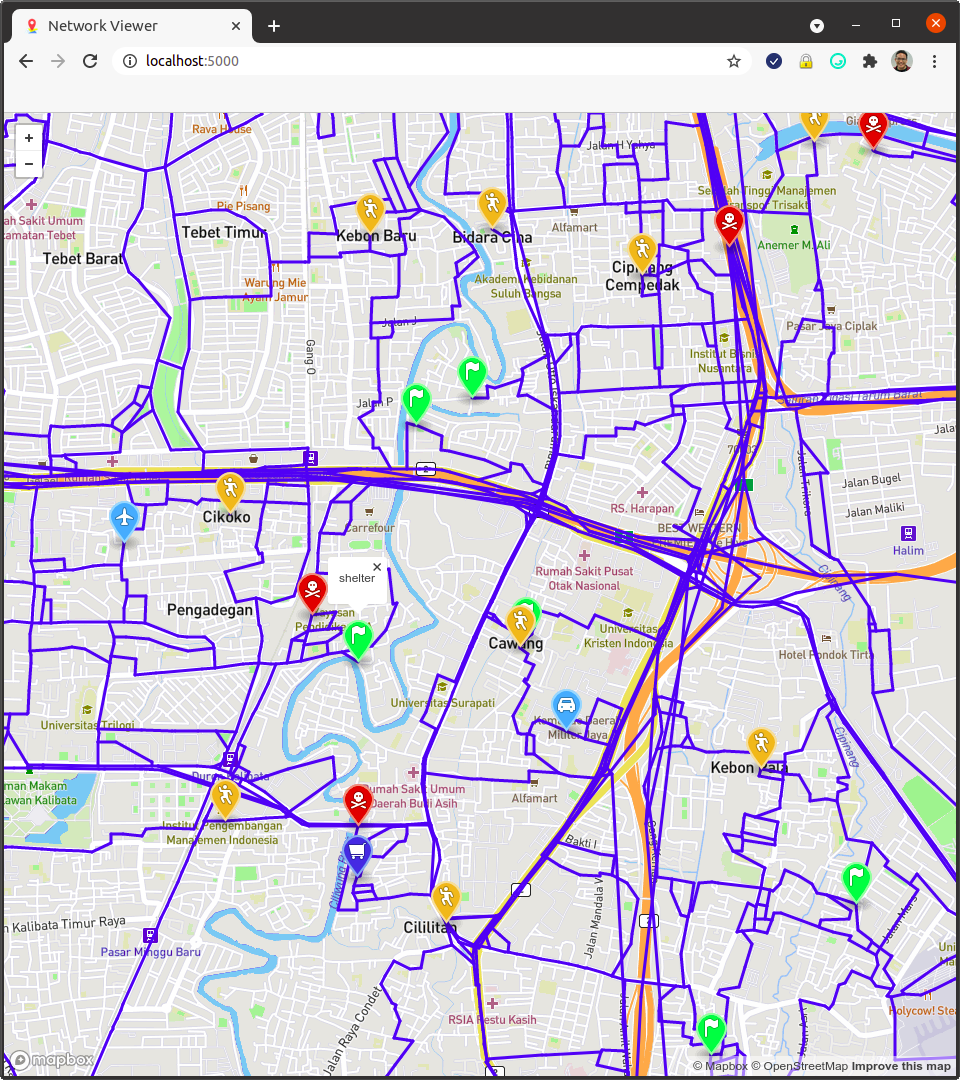
\includegraphics[scale=0.24]{subnetwork-visualization-zoom-1.png}}
\caption{Visualization of Jakarta's subnetwork during flood disaster}
\label{fig_jakarta_subnetwork_visualized}
\end{figure}


\section{Conclusion}

Our proposed system was able to generate route subnetwork for all given operations within considerable processing time. The time required to generate the subnetwork is affected by the number of POI and the area of the operation map. The bigger the number of POI and the area, the longer time required to generate the subnetwork.

Since the number of the POI in each operation is usually more than number of cores of CPU available in market, we'd suggest to integrate the method of running the shortest-path finding algorithm in Graphics Processing Unit (GPU) which has hundreds to thousands of cores \cite{harish2007accelerating}.


\bibliographystyle{IEEEtran}
\bibliography{references}

\end{document}
